\documentclass[10pt, a4paper, chapter]{oblivoir}
% \usepackage{apacite}
\usepackage{graphicx}
\graphicspath{ {./pics/} }
\usepackage{tabularray}
\usepackage{caption}
% \captionsetup{labelformat = empty}
\usepackage[style = apa, backend = biber]{biblatex}
\usepackage{fapapersize}
    \usefapapersize{210mm,297mm,25.4mm,25.4mm,30mm,25.4mm}
\pagenumbering{gobble}
% 챕터랑 숫자 같은 줄에 놓기 
\usepackage{titlesec}
\titleformat{\chapter}[hang] 
{\normalfont\huge\bfseries}{\thechapter}{1em}{} 

\setcounter{tocdepth}{5}
\setcounter{secnumdepth}{5}

\date{\large 2022~-~2학기}
\title{\Huge 일반사회논리및논술 실행연구 보고서\\
    \LARGE 수업을 통한 학생의 학습 효용감 제고 방안 탐구 및 관찰 방법 연구}
\author{\Large 2020127018 사회학과 손민우}

\addbibresource{ilsanon_paper_citation.bib}  

\setcounter{tocdepth}{2}
\setcounter{secnumdepth}{2}

\renewcommand{\hchaptertitlehead}{\thechapter}
\renewcommand{\thechapter}{\Roman{chapter}}
\renewcommand{\postchapternum}{.}
\renewcommand{\prechapternum}{~}

%bibliography 이름은 reference로 변경
\renewcommand{\bibname}{References}
\def\bibname{References}

\begin{document}
\maketitle
\tableofcontents*
\pagebreak
\chapter{실행 연구 계획}
    \section{선행 연구 분석}
    \cite{정민수2018교육과정}는 실행연구 방법론을 바탕으로 `교육과정-수업-평가-기록'의 일체화 수업 연구 과정을 구성하였다. 
    또한 동일한 글에서 `교실 수업에서의 일체화를 위해 교사는 수업을 계획하고 실행하는 과정에서 \textbf{목표 지향적}이어야 하며, 
    분명한 학습 목표를 염두에 두고 계획된 학습목표와 부합된 전략과 활동을 사용해야 한다''고 이야기 한다.\footnote{원문에서는 굵은 글씨 처리가 없었고 본 계획서에서는 의미를 강조하고자 추가함} 동일한 글에서 평가를 위한 준거 기준으로써 
    ``구조화''와 ``분류화''를 제시하는데, 구조화는 ``비대칭적인 권력관계'' 속에서 상징화된 정체성의 틀에 맞추어 의사소통이 진행되는 점을 
    이야기하고 분류화는 ``형성된 권력 구조''를 바탕으로 객체를 나누는 것을 의미한다. 이를 바탕으로, 수업 내부에서 교사와 학생 간의 
    의사소통이 진행되는 과정 속에서 구조화와 분류화의 정도를 제시함으로써 수업의 진행 방향을 이야기해볼 수 있을 것이며, 결정된 진행 방향은
    앞서 말한 학습 목표와 연관된 내용을 잘 조직화 할 수 있도록 구성하기 위해 어떠한 점이 요구되는지 검증할 필요가 있다고 느꼈다. 

    \cite{강대현2013사회과}은 교사의 전문성 발달에 관해 판단할 수 있는 통합적인 틀을 제시한다. 골자는 교사의 수업 내용 전달력, 교과의 전문지식 보유 여부,
    수업에 관한 성찰 정도 등이 종합적으로 교사가 가지는 역량에 영향을 미친다는 것이다. 중등교육에서 교사의 역할은 단순히 교과내용 전달에 그치는 것이
    아니라 학생 생활 전반과 진로 진학 지도까지 포함한다는 점을 고려해보았을 때, 교사는 교과 전문성에 더해 학생의 일상적이거나 특수한 갈등, 고민 상황에 대해서 
    올바르게 조언할 수 있고 `성찰하기 위한 틀'을 제시할 수 있어야 한다. 따라서 학생들이 수업 과정에서 가질 수 있는 수업과 직/간접적으로 관련되는 
    여러 고민들을 교사가 이해할 수 있는 방법은 없을지에 대해 생각해 볼 필요가 있을 것이다. 비슷한 맥락 속에서,
    \cite{한광웅2010사회과}은 ``예비교사의 수업전문성은 수업의 의미와 교사의 정체성 및 역량에 대해 근본적인 수준에서 반성하고,
    이를 수업실천의 맥락에서 실행할 수 있는 능력과 개방된 마음가짐을 가리킨다''고 하였다. \cite{leeEnglish}은 ``\dots 실행연구 주체로서 교사는 
    현장에서 학생들이 느끼는 문제점을 스스로 파악하고 주도적으로 해결방안을 탐색하여야 한다'', ``학생들이 진정으로 필요로 하는 해결책을 제시하기 위해서는 
    학생들이 당면하는 문제를 규명하는 행위가 실행연구 과정에서 시작점이 되어야 한다.''고 언급한다. 마찬가지로, 수업관련 정체성은 교사로서 아이들에게 무엇을 가르치고자 하는지, 수업의 목적을 어디
    에 두며 그것이 교사 자신과 어떻게 관련되는지를 탐색하는 것을 의미한다.(\cite{강지영2011국내})\\
    정리하자면 교사는 능동적으로 학생이 가지고 있는 문제를 파악하려 노력하는 동시에, 제 3자의 입장으로서가 아니라 학생 본연의 입장에서 
    필요로 하는 해결책을 고민해볼 필요가 있다. 

    사회과 연구는 연구 주제의 측면에서 `수업모형 및 교수·학습방법’ 토픽과 `교과서 및 교육과정’ 토픽에
    집중된 경향이 나타났다.( \cite{김재우2019텍스트})실행연구의 목적이 전문성 발달뿐만 아니라 연구자 개인의 
    내면적 성장과 사회구조 개선을 위한 것으로 다양화될 필요가 있다.(\cite{강지영2011국내}) \newline

    \noindent
    앞선 논의를 종합하면 아래와 같다. 
    \begin{itemize}[$\ast$]
        \item 교사 스스로 학생들의 반응과 행위를 확인하면서 교육 과정에 알맞게 학습 목표를 구성 및 조직하는 방법에 관해서 연구가 필요하다.
        \item 교사들이 학생들이 진정으로 필요한 요소를 어떻게 하면 찾아낼 수 있을 것인지 파악해야한다. 
        \item 단순히 교육과정을 잘 따라서 충실하게 ``학습''하도록 돕는 것에서 나아가 개별적인 학생의 학습 ``과정''에 대한 탐구가 요구된다. 
        \item 학생들과 관련된 교사의 ``탐구''에 있어서 교사가 가져야할 태도나 관찰 방법은 어떤 것이 적절할지 생각해보는 것이 바람직하다. 
    \end{itemize}

    이를 바탕으로 연구 질문을 구성하였다. 


    \section{연구 질문}
    \begin{enumerate}
        \item 어떻게 수업을 통해 학생들이 각자 학습 최적 경로를 찾을 수 있도록 도울 수 있을까?  \\ 읽기 자료를 통한 학습, 발표나 토의를 이용한 학습을 통해 적절한 학습 방법과 자료를 파악한다. 
        \item  이를 바탕으로 수업에서 나타나는 학생들의 상호작용이 실질적인 내용 학습에 어떠한 관계를 가질까? \\  수업 중에 제시되는 과제들을 통해 학생들이 갖고 있는 수업의 이해도와 사고의 깊이를 확인한다. 
        \item 다양한 관찰 방법을 통해 수업 중의 학생과 교사, 학생과 학생의 상호작용을 파악하면서 가장 유의미한 결과를 얻을 수 있는 관찰 방법은 어떤 것이 있을지 파악한다. 
    \end{enumerate}

    \section{연구 계획}

        \subsection{수업 계획}
        \textbf{학습목표}: 사회적 소수자에 대한 개념과 특성을 이해하고, 관련된 사회적 이슈에 대해 논의하며 학생 스스로 
        사회적 소수자와 관련된 문제에 대해 자신의 의견을 종합하여 개진할 수 있다. 
        \begin{enumerate}
            \item{도입}
            \begin{itemize}[-]
                \item 출석을 확인한다.
                \item 사회적 소수자 단원이 갖는 학습의 의의를 학생들에게 제시한다.
            \end{itemize}
            \item{전개}
            \begin{enumerate}
                \item 교과서 내용 학습
                \begin{itemize}[-]
                    \item 사회적 소수자의 개념과 예시를 흥미를 유발할 수 있는 영상자료와 함께 이해할 수 있도록 한다. 
                    \item 교과서의 학습활동을 통해 사회적 소수자에 대한 기본적인 개념을 학습할 수 있도록 하고, 이해 여부에 관해 발표를 유도한다.
                \end{itemize}
                \item 토론 학습
                \begin{itemize}[-]
                    \item 사회적 소수자의 상황에 대한 기사 자료를 읽기 자료로써 제시한다. \\ 논란이 있을 수 있으며 찬반의 여지가 나뉘는 내용을 제시하여 생각을 열 수 있도록 한다. 
                    \item \textbf{읽기 자료와 발표 및 토의를 함께 활용하는 동시에, 이를 각각 제시하여 효과를 확인 해보고자 한다.}
                \end{itemize}
                \item 심화 및 확장 학습
                \begin{itemize}[-]
                    \item 교과서에서 제시되어 논의의 바탕으로 이용한 사회적 소수자의 개념에 대해 재고해볼 수 있는 기회를 가질 수 있도록 한다. 
                    \item 사회 정체성이 다원화 되고 있다는 점을 고려하여, 학생의 단편적인 사회적 소수자 개념의 확장 가능성에 대해 중점적으로 논의한다. 
                \end{itemize}
            \end{enumerate}
        \item{평가 및 정리}
        \begin{itemize}[-]
            \item 학습지를 통해 본 수업의 내용을 정리하고 학생 스스로 생각과 기본 개념을 정리할 수 있도록 한다. 
            \item 찬반의 격화된 논의가 필요한 주제가 아니라 ``문제''를 해결하는 방안을 고민해봄으로써, 수업시간에 배운 내용을 실제 현실의 내용과 연결지어 생각할 수 있도록 한다. 
            \item 학생이 수업 내용을 받아들이고 공감하여, 최종적으로 수업의 가치를 스스로 파악하여 효용감을 가질 수 있는지 확인해보는 것이 필요하다. 
        \end{itemize}
    \end{enumerate}


        \subsection{자료 수집 계획}
        가능하다면 양적, 질적 자료 모두를 이용해서 결과를 도출하는 것이 조금이라도 더 유의미한 결과를 낼 수 있을 것이다. 추가적으로 자료 수집에서
        중점적으로 고려해야할 점은 학생이 수업 과정 중이나 수업 후에, 학생들이 ``원하는 바''를 이해하고 짚어낼 수 있도록 돕는 요소를 파악해야한다는 것이다.
        \begin{itemize}[-]
            \item \textbf{양적 자료}
            

            수업 대상의 학생 수가 제한적이므로, 양적 자료를 이용해서 많은 결과값을 얻을 수 없다는 점을 고려하면, 학생들이 
            수업을 겪으며 느끼는 감상을 간단히 수치화하여 수집하는 것이 유의미하다고 판단했다. 따라서 양적자료는 수업 직후에 
            학생이 수업의 각 과정에서 느꼈던 ``향상감''이나 ``어려움'' 등을 측정할 수 있는 점수를 수집하고자 한다. 
            \item \textbf{질적 자료}
            

            수업 전, 중, 후에 관찰을 통해서 학생들이 수업에 집중하는 정도나 수업에 열의 등을 확인하고자 한다. 수업 중에 
            제시되는 학습지에 대한 충실도 여부와 앞서 이야기된 양적 자료를 간단히 비교해보고자 한다. 수업을 전개해나가는 과정 속에서 
            학생의 사고가 심화되는지, 혹은 학생이 수업의 내용을 받아들이지 못하고 사고 자체도 정체가 되는지 등 다층적인 면에서 학생이 
            이용한 학습지를 분석하고자 한다. 
        \end{itemize}

\pagebreak

\chapter{수업 진행 과정 및 수업 분석} % 자기 평가 
%수업의 취지와 강조점, 수업 피드백 분석 
    \section{수업 진행 과정 개요}
    \begin{enumerate}
        \item \textbf{도입}
        
        본 실행 연구를 위한 수업 시연은 11월 21일 오후 5시부터 약 1시간 동안 진행되었다. 수업은 먼저 담임 교사가 학생들이 수업 내용과 관련된 생각들을 스스로 해볼 수 있도록 ``포스트잇''을 활용해서 각자의 생각을 써보도록 하는 것으로 시작되었다.~%
        이를 통해 수업을 통한 학습 이전에 학생들이 갖고 있는 지식을 확인하고 수업에서 다룰 개념의 의의를 스스로 생각해볼 수 있는 기회를 마련했다. 
        \item \textbf{전개}
        
        그 다음은 교사가 수업 내용인 `사회적 소수자'에 관한 교과서 개념을 영상 자료와 함께 제시했다. 지도한 교과서 개념을 바탕으로 제작한 읽기 자료를 이용해 토론 학습을 진행했다. 이는 수업 내용과 관련된 읽기 활동과 토론을 병합하여 진행하는 방식으로 학습 내용에 대한 이해를 도울 수 있도록 하기 위함이었다.
        토론을 통해서 스스로 생각한 부분에 더해 조원들이 갖고 있는 생각을 들음으로써 다양한 생각과 입장을 이해할 수 있는 기회를 갖도록 하였다. 
        토론 종료 후 학생들이 가진 생각과 입장들을 발표할 수 있는 기회도 마련하였다.
        \item \textbf{마무리}
        
        추가적으로 한 개 영상을 더 제시하고, 수업 시간동안 학습하내 내용을 스스로 복기하고 심화할 수 있는 기회를 학습지를 통해 제공했다.
        최종적으로는 `사회적 소수자' 개념의 확장성과 다양성을 이해하여 사회과학적 개념이 갖는 특성 또한 암묵적으로 이해할 수 있도록 했다.
        학생 스스로 수업에서 배운 개념을 정리하는 과정에서 특정 입장에 경도되지 않고 서술할 수 있도록 질문을 구성하였다.
    \end{enumerate}

    \section{수업 분석}
    \begin{enumerate}
        \item \textbf{도입}
        
        학생들의 피로감이 적은 수업 시작지점에 참여를 유도하였고, 이에 따라 다양한 대답을 얻을 수가 있었다. 
        또한 학생들이 수업에서 다룰 개념인 `사회적 소수자'에 대해서 스스로 능동적으로 생각할 수 있는 기회를 제공하였다는 점에서 적절한 도입이었다고 판단했다.
        \item \textbf{전개}
        
        영상과 함께한 `사회적 소수자'의 개념 제시는 관련 내용에 대해서 지식이 없는 학생들도 잘 이해할 수 있었을 것이라고 생각한다.
        그러나 다양한 학습 활동에 대한 학생들의 태도와 생각들, 그리고 행태를 파악하는 것에 중점을 두어 짧은 시간 동안 학생들에게~
        큰 부담을 주었다고 생각한다.

        그럼에도 불구하고 읽기 자료를 올바르게 이해하고 토론에 적극적으로 참여한 학생이 많았고, 이러한 학생들을 통해서 동일한 조에 속한 학생들이 
        스스로 이해하지 못한 부분에 대해 도움을 얻고 자신의 입장을 재정리할 수 있는 기회를 얻었을 것이라 판단한다. 

        읽기 자료와 토론 학습을 함께 진행하는 것이 아니라, 읽기 자료에 따른 학생의 생각을 개별적으로 파악해보는 것이 더 낫다고 판단했다. 토론학습에 대해서는 주제 제시를 읽기 자료를 바탕으로 하기보다는,
        학생들이 이해하고 받아들이기 쉬운 영상 자료를 통해 주제를 파악하도록 유도하는 게 더 바람직 했을 가능성이 있다.

        토론 내용을 학생들에게 물어 발표하는 과정에서 학생들의 자발적인 지원을 기대하기 보다는, 토론 이전에 학생들에게 발표 가능성에 대해 확실하게 
        주지시키고 토론에 임하여 좀 더 적극적인 토론이 될 수 있었을 것이라 추측한다.  
        \item \textbf{마무리}
        
        소수를 제외하면 마무리 학습지 활동에서 수업 시간에 배웠던 `사회적 소수자' 개념을 이용해 영상 자료의 내용을 스스로 해석할 수 있음을 확인했다. 
        또 각자의 경험을 서술함으로써 학생 주변의 상황에서 ``교과 개념''을 적용할 수 있는 상황을 파악하며, 교과 내용과 현실을 연결할 수 있음을 묵시적으로 
        파악할 수 있도록 하였다. 

        마지막으로 학생이 수업을 통해 느낀 점을 서술하게 함으로써, 다시 한 번 학습한 내용을 스스로 상기할 수 있도록 하였다. 

    \end{enumerate}

\noindent
    본 수업 시간에 지도한 `사회적 소수자' 개념을 지속적으로 반복하여 학습하고 적용해봄으로써 학생 스스로 개념의 이해를 확인할 수 있도록 하는 방식을 취했다. 
    토론 학습을 통해서는 스스로 이해$\cdot$적용한 개념이 적절한 것인지 아닌지 다른 학생과의 비교를 통해 판단함으로써, 학생이 스스로 학습 상황을 진단하며 
    수업 내용을 능동적으로 이해할 수 있도록 했다.  

    \section{수업 시연 피드백 분석}

    수업 시연 후 피드백 설문을 통해 얻을 수 있었던 수업 시연에 대한 의견을 종합하면 아래와 같다. \newline

\noindent
    수업에서 다룬 `사회적 소수자'의 개념이 제시된 방식이나 준비된 자료가 가진 효용성에 대한 비판은 적었다. 또한 수업에서 이루어진 개념에 대한 설명, 수업을 통해 학생들에게 지도하고자 한 학습 목표 와 같은 ``교과 수업''의 내용을 학생들에게 전달하는 것은 성공적이었다고 볼 수 있다. 
    또한 학생들이 수업의 내용을 수동적으로 받아들이지 않고 능동적으로 스스로 사유하며 이해할 수 있도록 수업이 구성되었다는 의견도 있었다. 
    다양한 자료를 통해서 학생들의 수업 참여를 유도했고 교과 개념의 기본적인 이해를 돕는 것에서 나아가, 이해한 개념을 바탕으로 스스로 사례에 적용하는 연습을 통해 이해를 심화할 수 있는 기회를 제공했다는 점이 이야기 되었다. \newline

\noindent
    동일한 피드백 설문을 통해서 얻을 수 있었던 수업 시연의 아쉬운 점을 정리하면 아래와 같다. 
    \begin{itemize}
        \item \textbf{학생들의 수업 부담이 크다.}
        
        수업 받는 대상이 일반사회 과목인 사회문화 과목을 학습하는 고등학교 2학년 학생임을 가정했을 때, 수업 시간동안 학생들이 받은 질문들은 답을 내기가
        쉽지 않다는 점을 알 수 있다. 

        제한된 시간 내에서 학생들에게 여러 가지 자료를 제시하고, 많은 질문들을 제시함으로써 학생들이 갖는 지적$\cdot$시간적 부담이 크게 느껴졌다.

        \item \textbf{발표를 유도하는 방식이 적절치 못하였다.}
        
        일반적인 대한민국의 교실 상황에서는 특정한 학생 일부들만 발표를 지속적으로 하게 되고, 다른 학생들은 발표를 하려 자원하지 않다는 점이 고려되지 못했다. 
        토론을 내용을 바탕으로 학생들의 의견을 요구하는 것은 좋았지만, 의견 요구에 있어서 발표를 유도하는 방식은 좋지 못했다. 

        \item \textbf{학생들의 의견과 생각에 대한 피드백이 없다.}
        
        토론과 학습지 활동으로 스스로 고민하여 떠올려 본 생각들에 대해서 학생들이 자신이 생각한 의견에 대해서 선생님의 확인을 받을 수 있는 기회가 거의 없었다.
        학생들의 생각의 변화를 야기하기 위해서는 학생들이 가진 생각들을 세심하게 추적하고 꼬집어 가며 수업을 진행할 필요가 있다. 

        \item \textbf{수업 학습지의 질문들이 생각의 단계를 밟아 나가도록 도움을 주지 못하고, 의도가 불명확하게 느껴진다.}
        
        특히 `이상한 변호사 우영우' 관련 영상을 시청한 뒤에 주어진 질문들은 학생들이 앞선 개념과 논의들을 제대로 이해하였다는 가정을 바탕으로 
        이루어져 있다. 이로 인해서, 앞선 시간에 개념을 정립하기 어려웠을 학생들은 애로 사항을 겪을 가능성이 크다.

        토론을 위한 학습지 구성에서도 토론 주제에 대해서 명확하게 제시해주지 않고 읽기 자료와 학습지를 통해 학생 스스로 파악하도록 한 점이 문제가 될 수 있다.
    \end{itemize}
\noindent
    본 수업 시연을 바탕으로 하는 실행 연구가 서로 다른 학습 자료가 가진 효용을 비교하고자 한 점 때문에, 다양한 학습 자료를 제시할 수 밖에 없었다. 이로 인해서 학생들이 느끼는 부담이 커질 수 밖에 없었을 것이라 판단된다. 
    또한 교실 현장의 상황과 환경을 고려하지 못하고 수업이 설계된 부분이 존재했고 학생들끼리 의견을 나누고 스스로 생각해보는 활동이 위주로 되어 교사가 개입하는 부분이 적었다. 
    따라서 교과 내용을 올바르게 이해하고 있는 교사가 직접적으로 지도하는 부분이 적어져 학생들이 교과 개념을 이해하고 활용하는 것에 있어서 일반적인 수업보다 더 큰 부담을 짊어졌을 것이라 생각된다. 즉, 수업 내용에 대한 적절한 피드백이 모자라서 학생들의 학습 부담을 가중시켰을 가능성을 배제할 수 없다는 것이다. 

    비슷한 문제로 수업 관련 내용과 자료를 이해하지 못한 학생의 경우에는 주변에 도움을 줄 학생이 없는 경우에는 계속적으로 수업을 따라가지 못하는 악순환이 발생할 수 있을 가능성이 존재했다. 
    물론 조별 토론 시간에는 교생이 개입하여 학생들간의 논의를 조절할 수 있도록 했지만, 수업 특성상 각 교생이 갖는 능력이 상이하여 학생들이 갖는 개별적 어려움을 모두 해소해주기는 힘들었다. 

    다양한 관점을 통해 제시된 개념을 바탕으로 사례를 해석할 수 있게 수업을 이끌어가도록 노력했지만 모든 학생들이 그렇게 느끼지는 못하고, 일부 학생은 수업에서 제시한 사례의 해석 방향이 정해져있다고 느꼈다. 



\chapter{자료 분석}
수업 이후 수업에 참가한 인원들을 대상으로, 수업에서 사용된 학습 자료와 활등들이 수업의 이해에 어느 정도로 도움이 되 었는지 확인해보고자 하였다. 수업에서 이용된 자료와 활동인 `읽기 자료', `토론 활동', `영상 자료', `학습지'의 네 가지 자료 및 활동이 수업을 직접 참가한 인원들이 느끼기에, 스스로의 학습에 도움을 준 정도를 알아보고자 했다. 

리커트 척도를 이용해서 `1점이 가장 불만족'스럽고, 5점이 `가장 만족스럽다'를 기준으로 하여 설문을 실시했다. 또한, 리커트 척도를 통해 부여한 점수에 대한 구체적인 이유를 질의하여 이를 바탕으로 분석을 실시했다. 리커트 척도 점수를 기준으로 정리된 자료는 표~\ref{tab:avgandsd}와 같다. 
% note 추가 
%%%%
\begin{longtblr}[caption = {수업 후 학습자료 효용감 설문\\%
    설문에 응답한 21명에 대해서 값을 구함}, entry = {},
    label = {tab:avgandsd}, remark{참고}={\small 설문점수: 평균(표준 편차)\\1점: 전혀 도움이 되지 않았다, %
    2점: 별로 도움이 되지 않았다\\3점: 잘 모르겠다\\ 4점: 어느 정도 도움이 되었다, 5점: 많은 도움이 되었다}]{colspec = {}, row{1} ={font=\small\bfseries} }
    \hline
    읽기 자료 & 토론 활동 & 영상 자료 & 학습지 \\
    \hline
    4.43(0.507) & 4.29(0.784) & 4.10(0.889) & 4.10(0.768) \\
\end{longtblr}
%%%%%
\begin{figure}
    \captionsetup{justification=centering} % catpion align ! 

    \begin{minipage}{0.45\linewidth}        
        \centering
        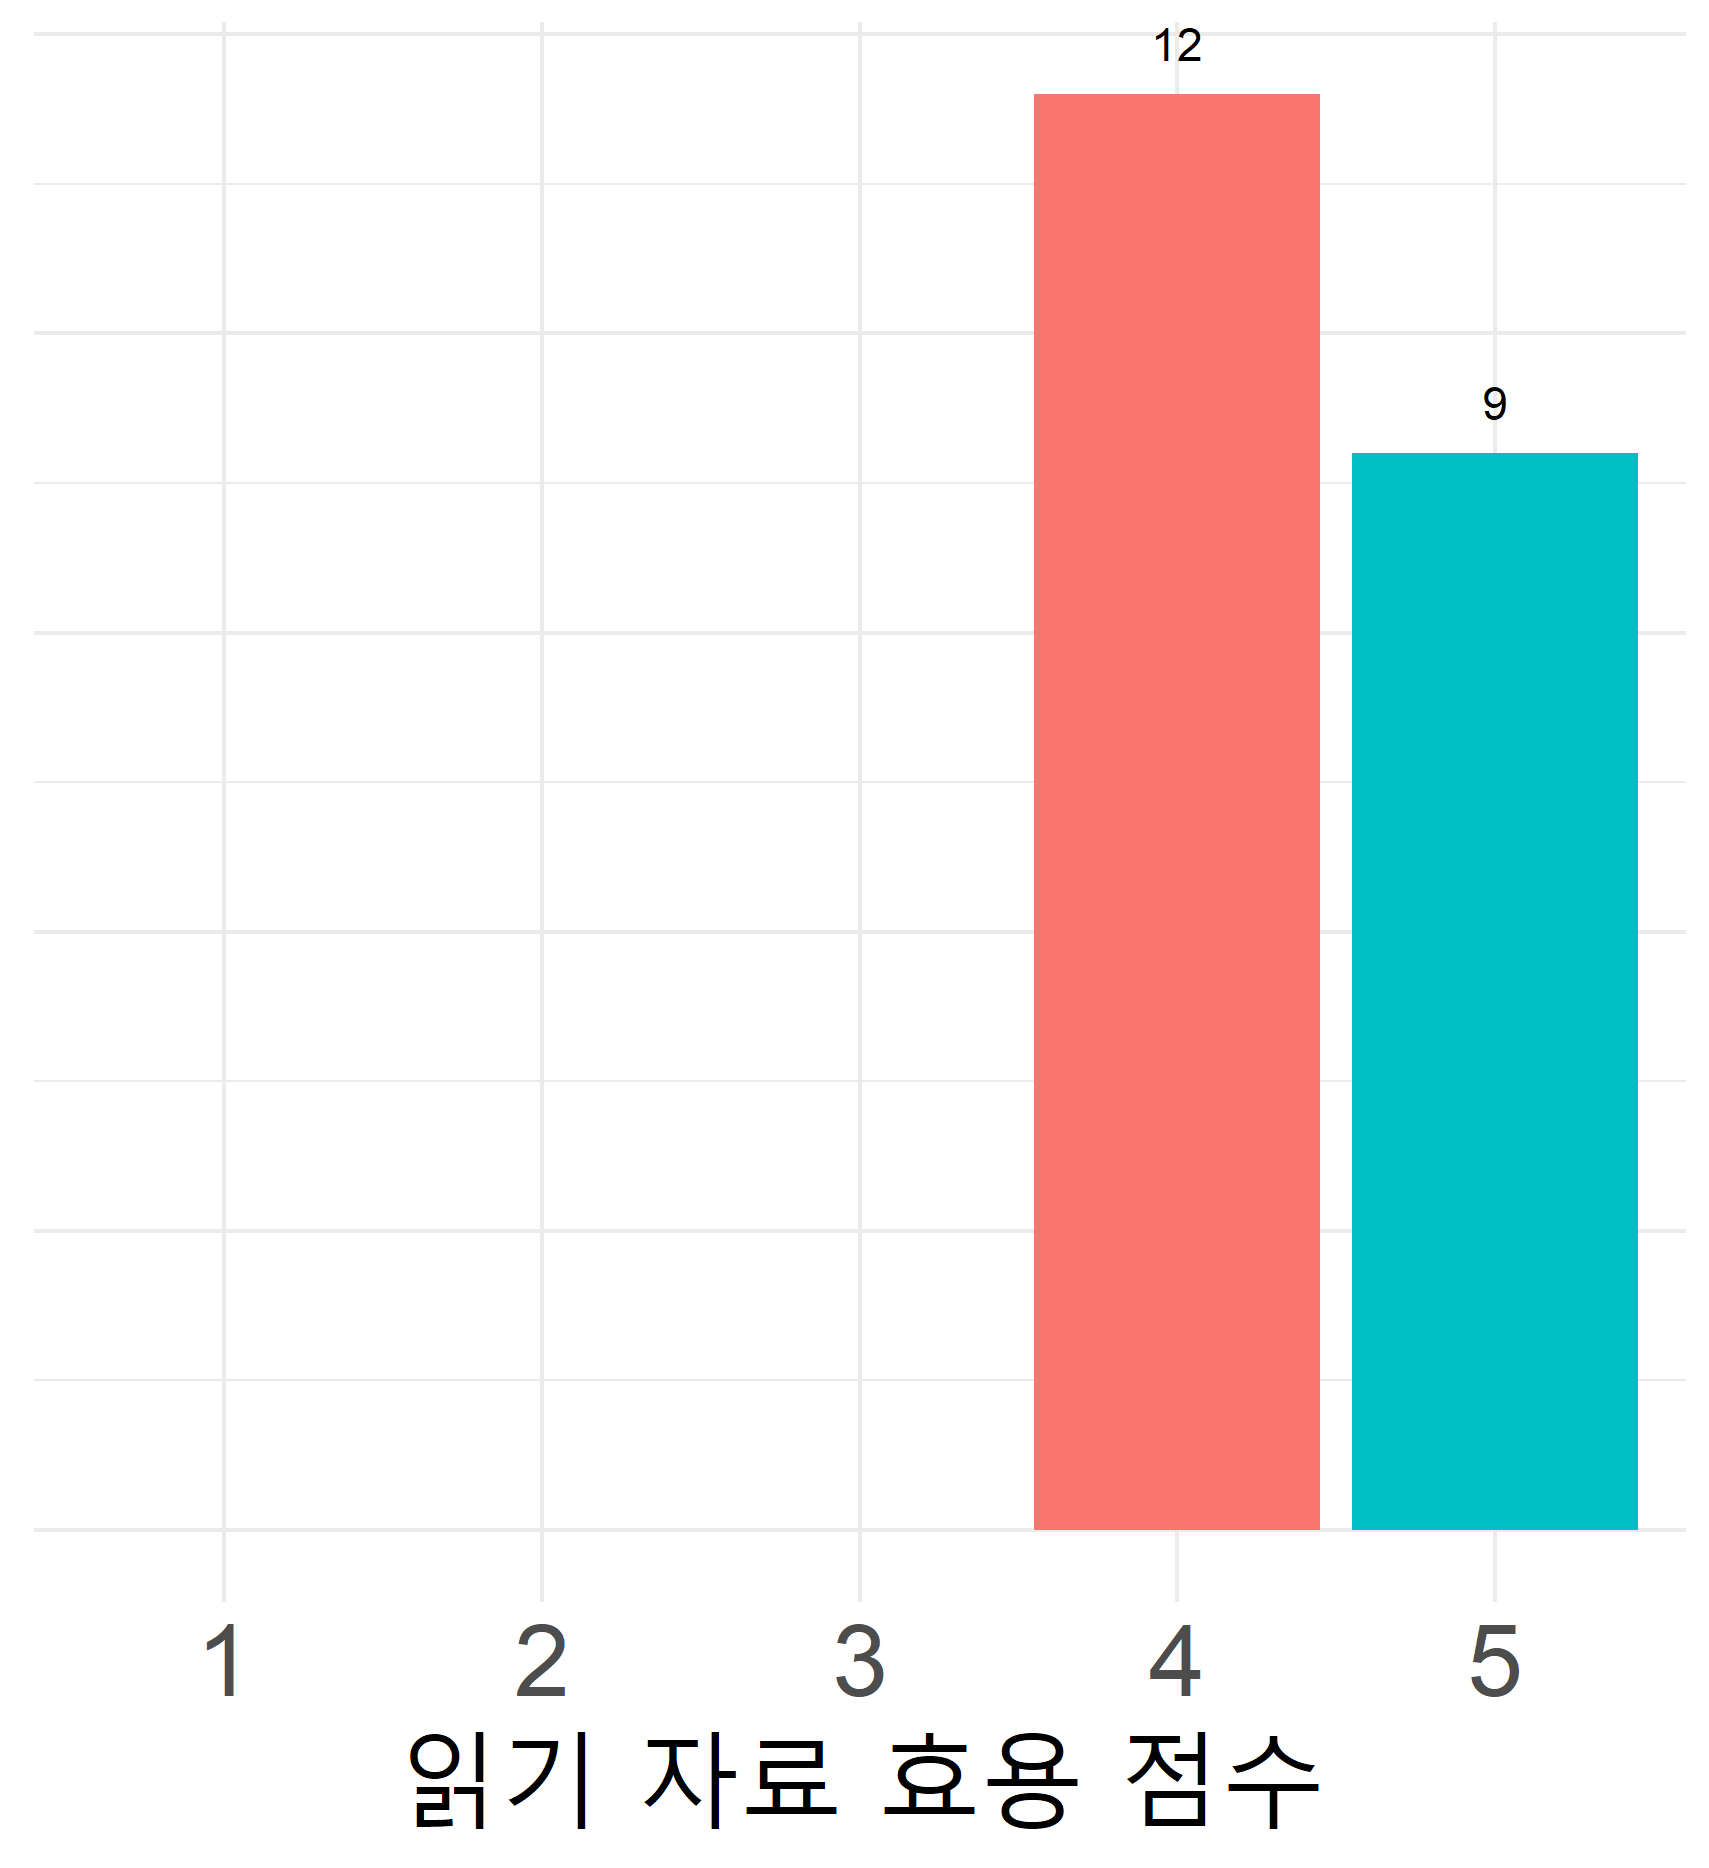
\includegraphics[height = 4.6cm, width = 0.75\linewidth]{reading.png}
        \caption{4점: 12명, 5점: 9명}
        \label{reading}
    \end{minipage}
    \hspace{0.05\linewidth}
    \begin{minipage}{0.45\linewidth}        
        \centering
        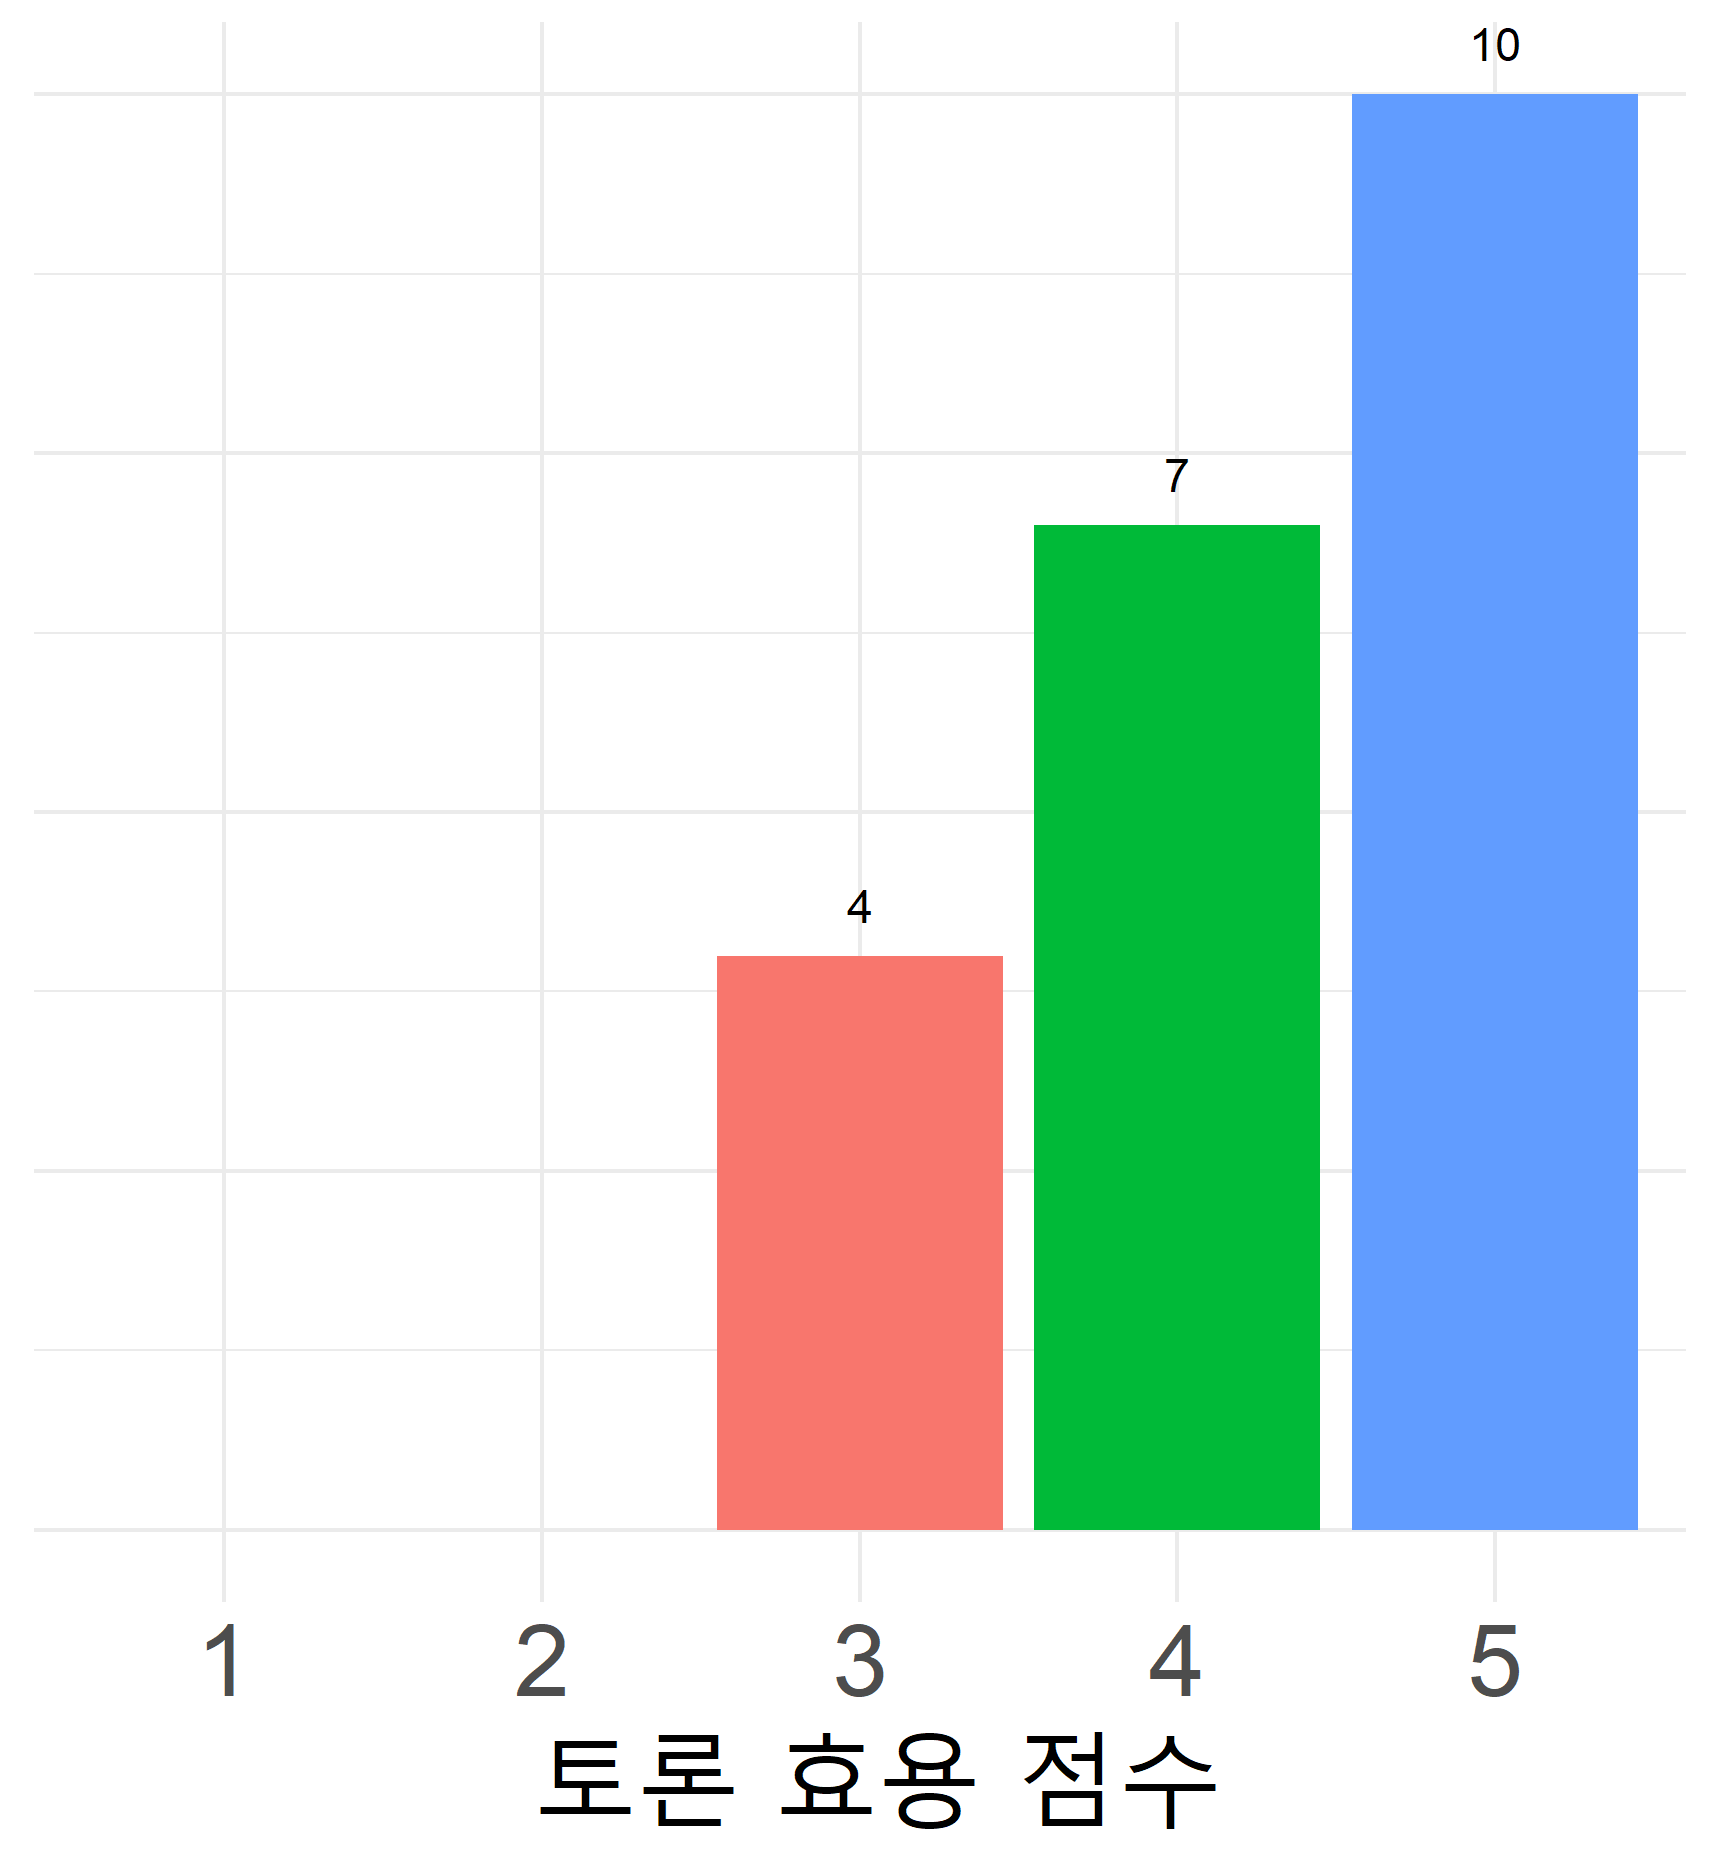
\includegraphics[height = 4.6cm, width = 0.75\linewidth]{debate.png}
        \caption{3점: 4명, 4점: 7명, 5점 10명}
        \label{debate}
    \end{minipage}
    \newline
    \begin{minipage}{0.45\linewidth}        
        \centering
        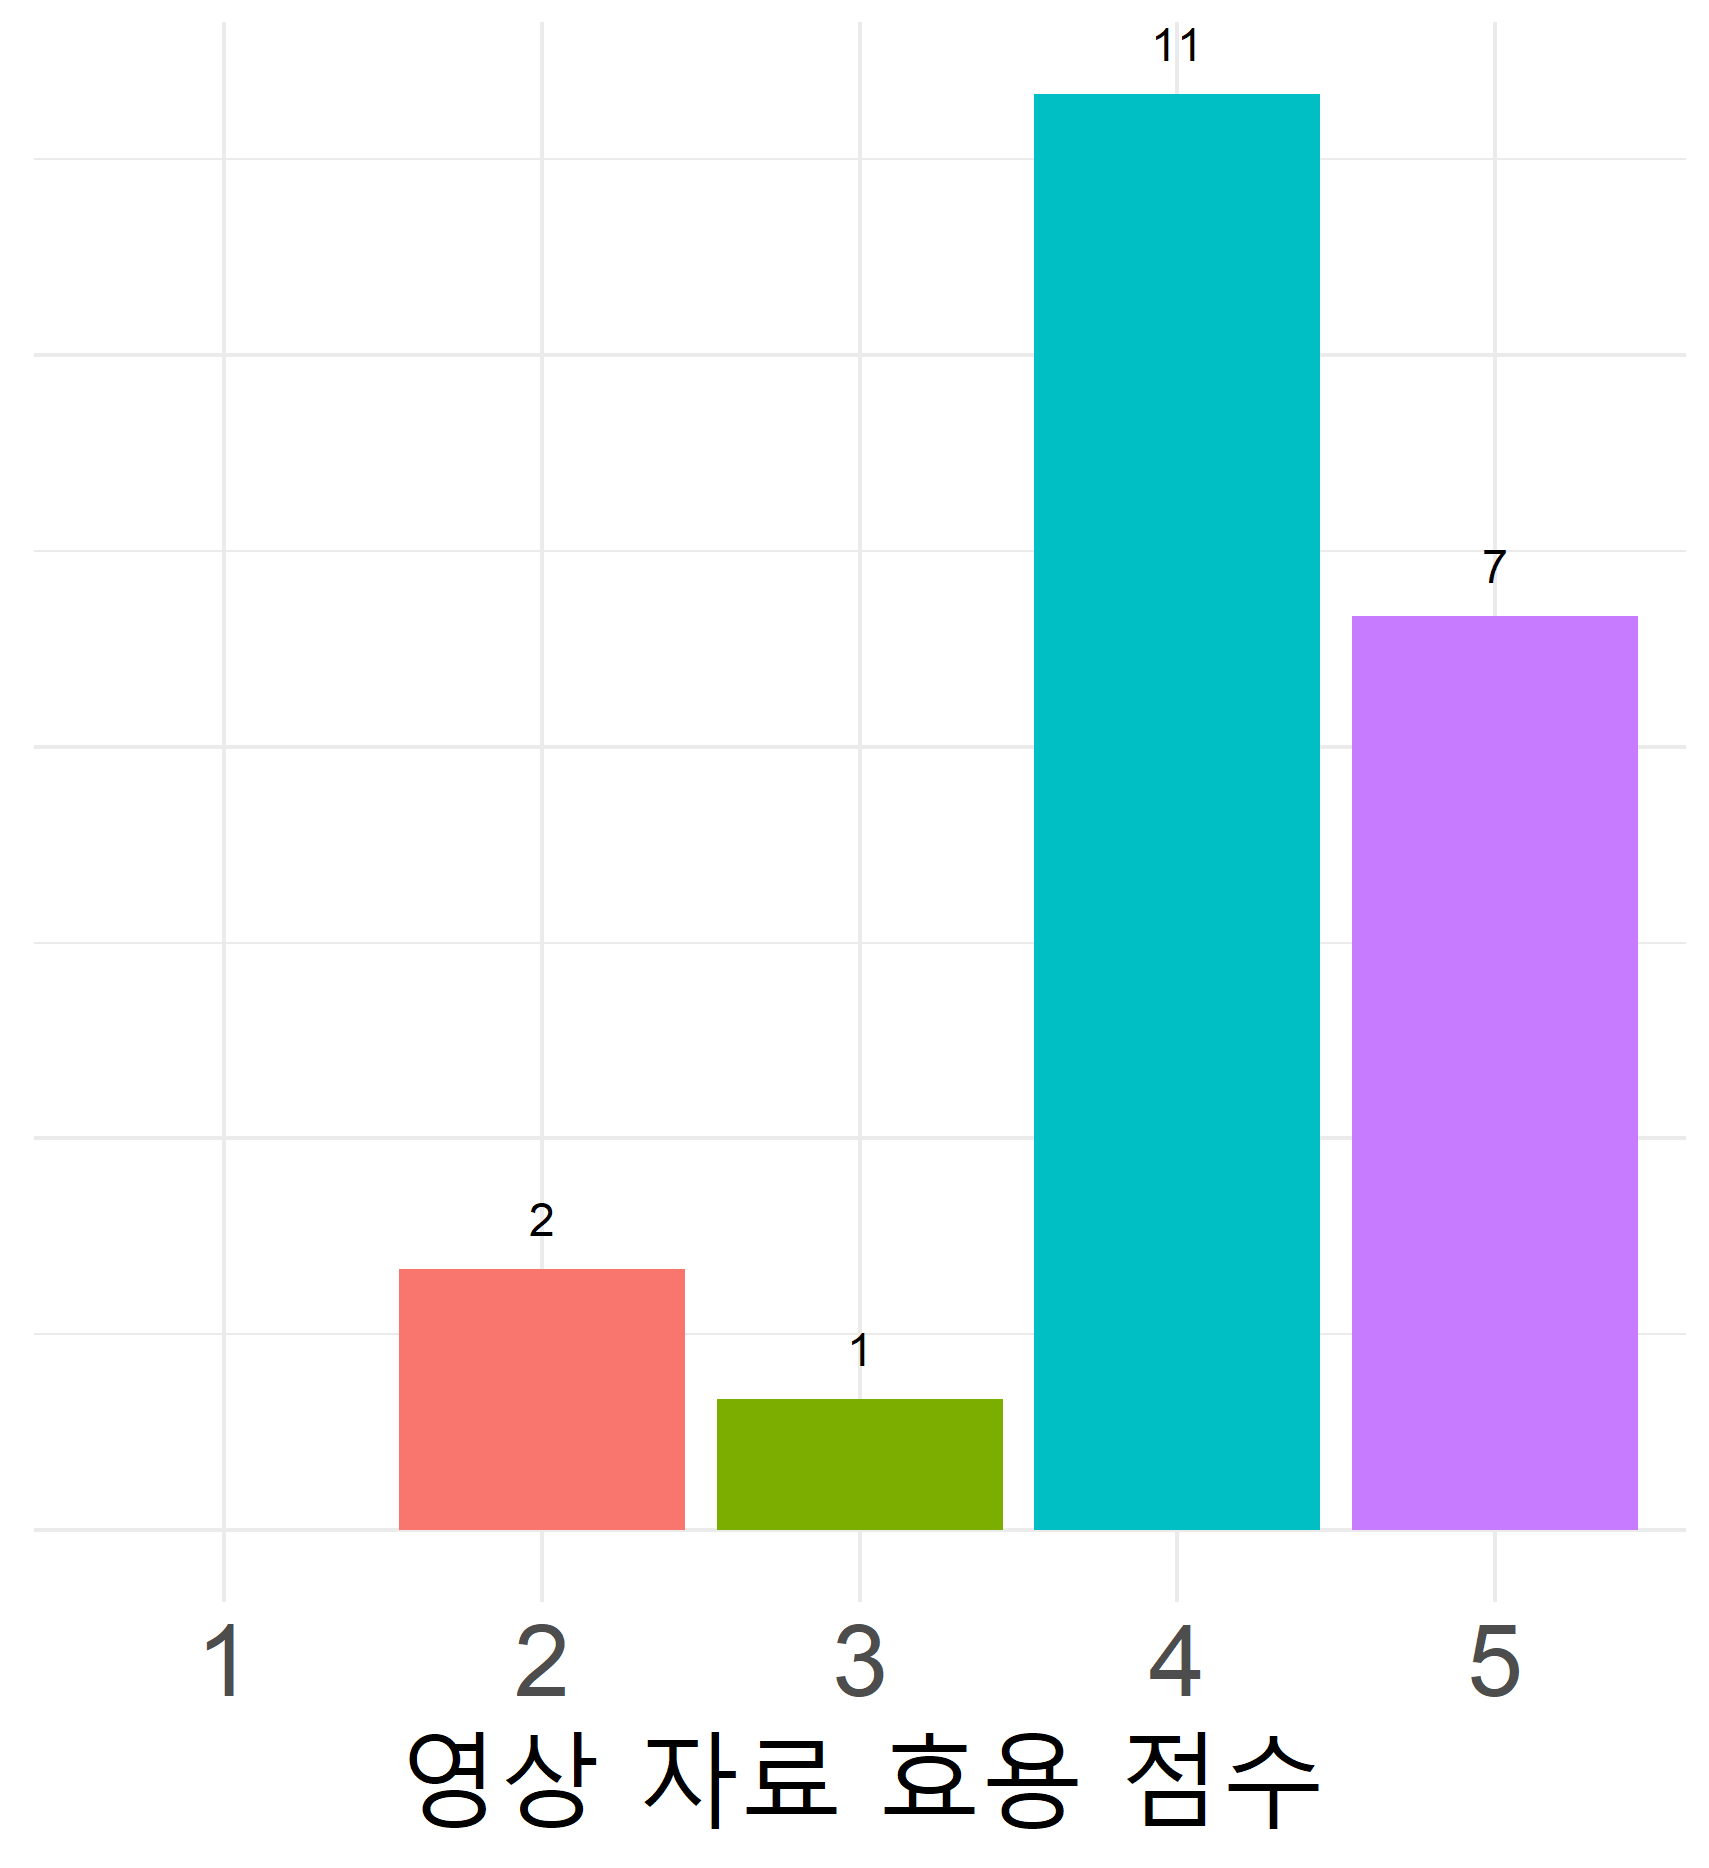
\includegraphics[height = 4.6cm, width = 0.75\linewidth]{video.png}
        \caption{2점: 2명, 3점: 1명, 4점: 11명,\\5점: 7명}
        \label{video}
    \end{minipage}
    \hspace{0.05\linewidth}
    \begin{minipage}{0.45\linewidth}        
        \centering
        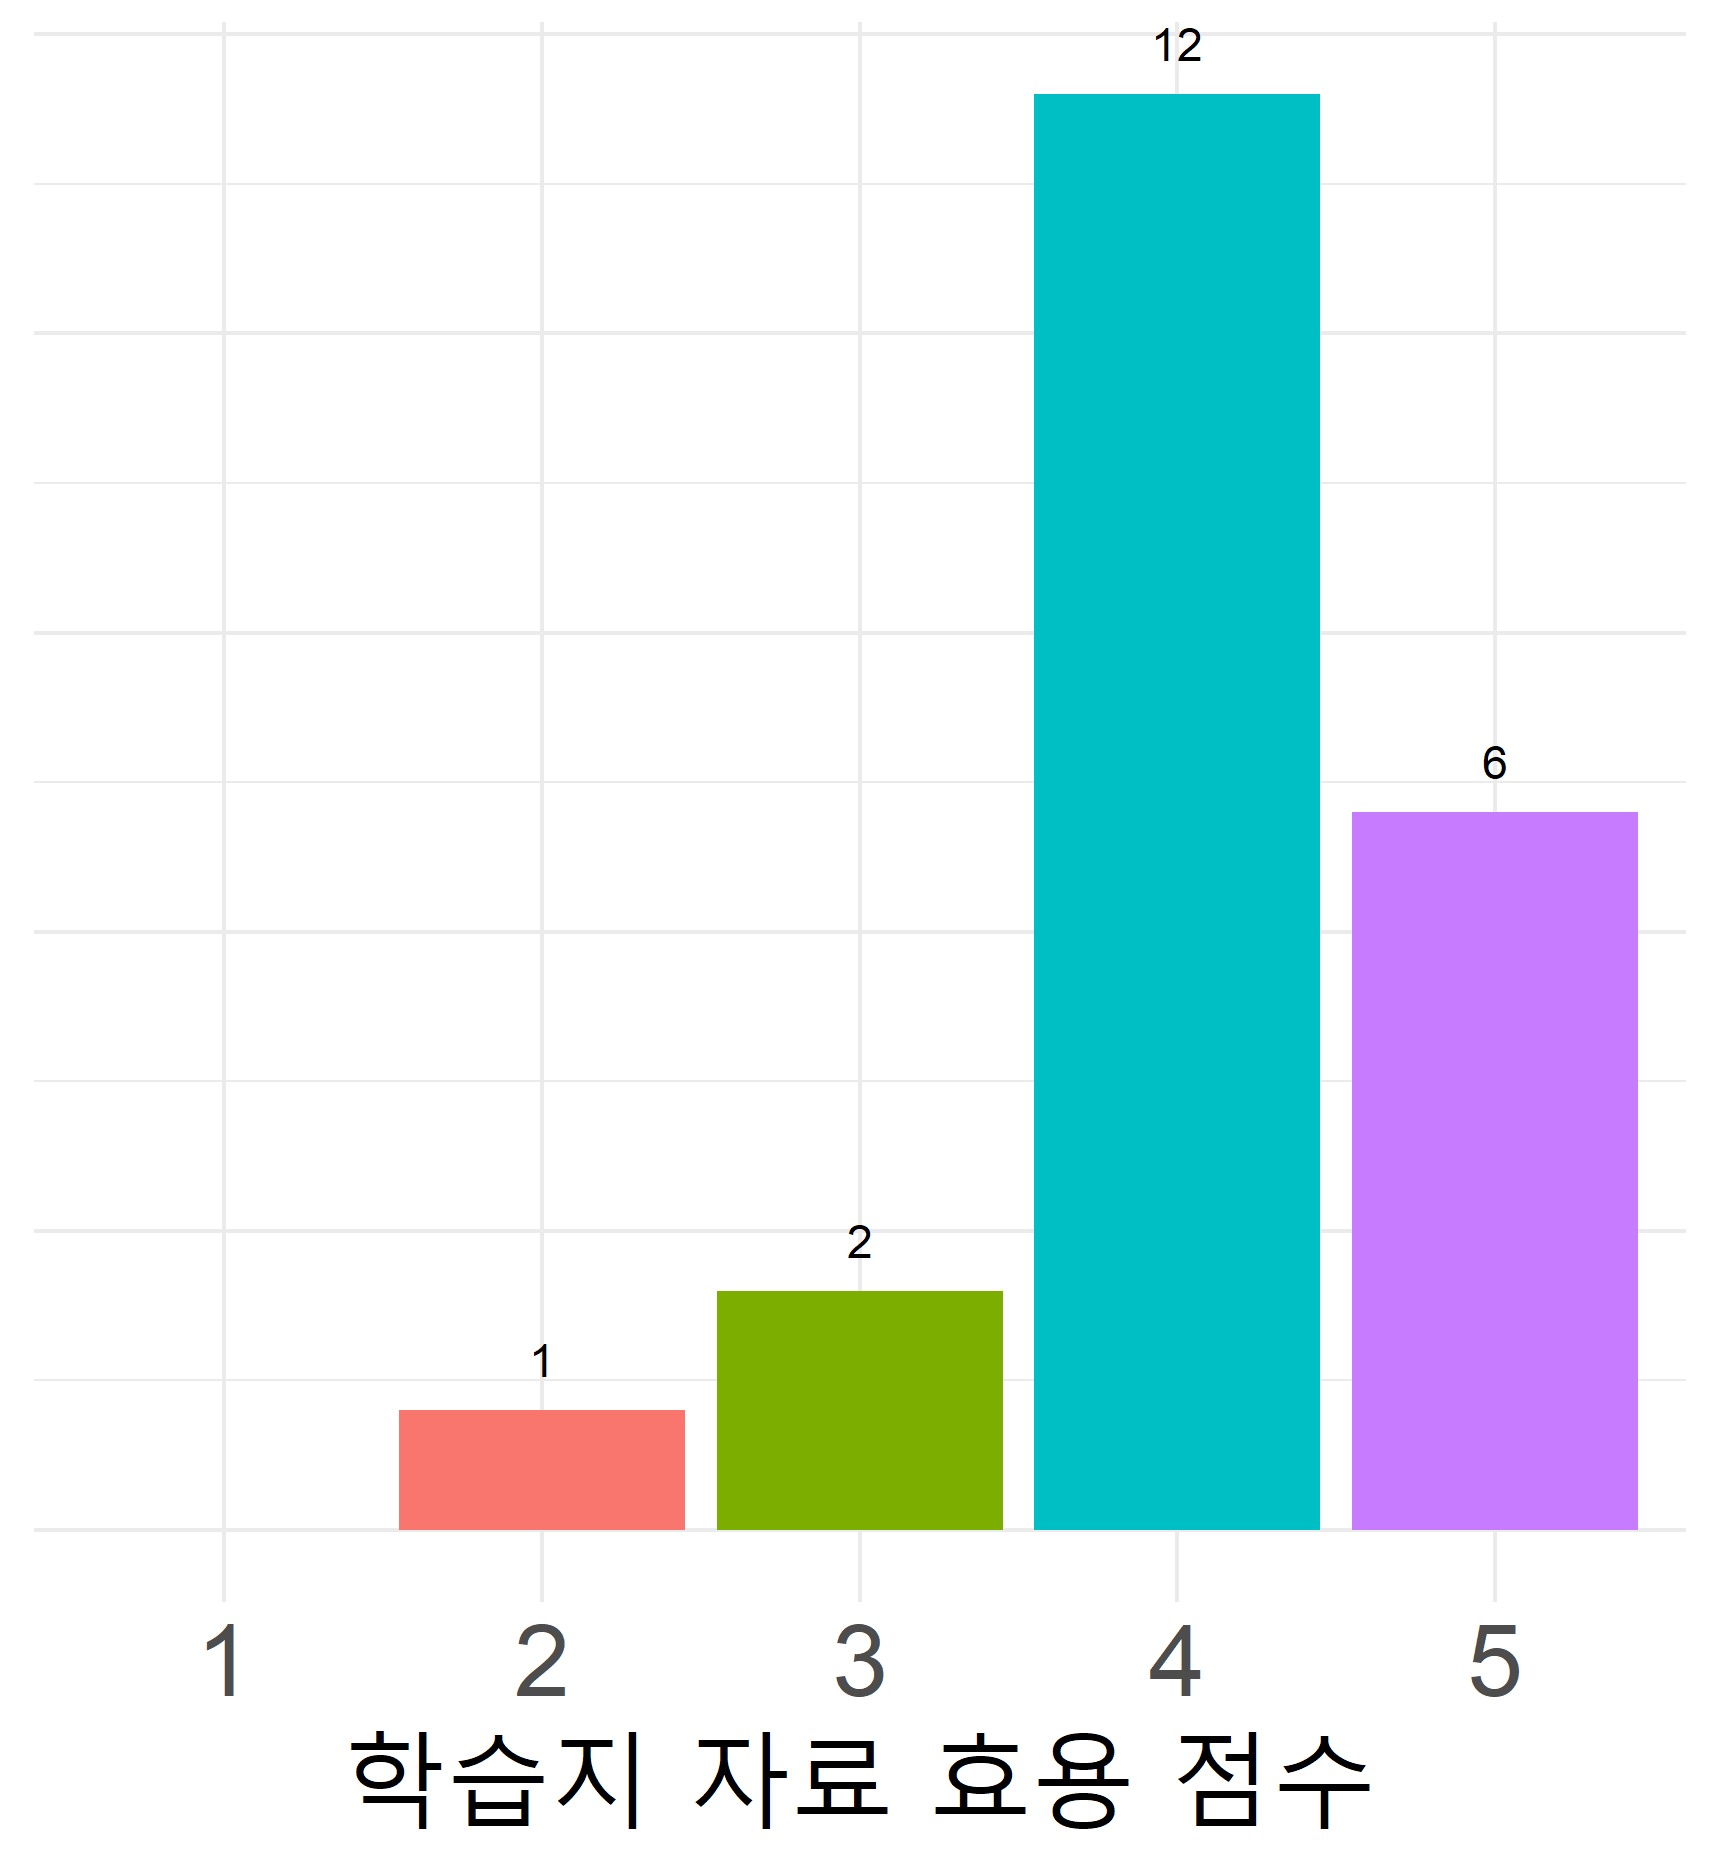
\includegraphics[height = 4.6cm, width = 0.75\linewidth]{material.png}
        \caption{2점: 1명, 3점: 2명, 4점: 12명,\\5점: 6명}
        \label{material}
    \end{minipage}
    
\end{figure}
\noindent
각 설문 자료의 최빈값은 읽기 자료 4점(그림 \ref{reading}), 토론 활동5점(그림 \ref{debate}), 영상 자료 4점(그림 \ref{video}), 학습지 4점 (그림 \ref{material})
이며 평균은 표 \ref{tab:avgandsd}에 나타나 있다. 이를 참고한다면, 각 자료들은 일반적으로 학생들에게 학습 이해에 도움을 줄 수 있는 자료로 인식되었다고 볼 수 있다.
아래의 점수 분포를 참고하면, 읽기 자료(\ref{reading})와 토론 활동(\ref{debate})에 대해서는 불만족인 의견(1점, 2점)이 전혀 없었으며, 나머지 영상 자료(\ref{video})와 학습지(\ref{material})에 대해서는 불만족인 의견이 각각 2명, 1명이 있었다.

영상 자료에 대해 2점을 준 두 명은 모두 영상 자료와 관련해서, 
수업 시연 과정에서 사용되었던 특정 영상(``이상한 변호사 우영우'' 드라마의 클립 영상)에 대한 배경설명의 부족이나 영상 속 이야기의 특수성을 지적하였다. 즉, 수업 시연 과정에서 선택한 
영상 `자료'의 적절성을 문제를 삼았으며 `영상' 자체의 효용성을 문제 삼지는 않았다. 3점(잘 모르겠다) 부여한 1명은, 수업 내용과 영상의 내용 간 연결성이 부족하다는 점을 지적하며 
앞서 언급한 것과 유사하게 영상 `자료'에 대한 `설명'에 관한 문제를 지적하였다.

학습지 설문에 대해 2점과 3점을 부여 세 명은 학습지에 부여된 문제 해결을 위한 가이드 라인의 부족,
학습지 속의 질문이 가진 다양성의 부족, 학습지의 난이도 문제를 지적하였다. 앞선 영상 자료의 
설문에서와 마찬가지로 `학습지'의 효용성을 문제 삼기보다는 학습지의 `구성'에 대해서 문제를 지적하며 학습지가 수업 진행에 가질 수 있는 효용성을 부정하였다고 보기는 어렵다. 

마지막으로 토론에 대해서는 4명이 `잘 모르겠다'고 답하였으며, 한 명의 인원은 수업에 참가하지 못하였기에 배제하고 언급하고자 한다. 따라서 나머지 3명 중 2명은 각각 토론 주제의 부적절성, 1명은
토론 과정 속에서 학생들의 주장을 듣고는 토론 활동이 실질적으로 학생이 `기존에' 가지고 있는 능력만을 활용하는 정도에 그치게 된다고 지적하였다. \newline

\noindent
각 자료와 활동이 갖는 효용성에 대한 긍정적인 답변을 요약$\cdot$정리하면 아래와 같다. 
\begin{enumerate}
    \item \textbf{읽기 자료}
    
    수업의 핵심인 `사회적 소수자' 개념을 적용하고 관련된 실제 사례 속에서 찬성/반대 의견을 확인하여 교과 개념을 실생활에서 적용될 수 있는 
    사회참여적 성격을 이해할 수 있었다. 
    \item \textbf{토론 활동}
    
    다른 조원들의 이야기를 들으면서 다양한 관점을 익힐 수 있는 기회가 되었고, 새롭게 들을 수 있었던 관점들을 바탕으로 
    자신 스스로의 입장을 재정립할 수 있는 기회가 되었다. 
    \item \textbf{영상 자료}
    
    읽기 자료와 유사하게 실생활에 적용할 수 있는 가능성에 대해서 다시금 확인할 수 있었고, 수업 시연 과정에서 중점적으로 다루었던 
    `사회적 소수자'와 `사회적 약자'의 개념을 더 명료히 이해할 수 있는 기회가 되었다. 

    자주 접하게 되었던 인물(인기 드라마의 주인공)을 통해서 읽기 자료에 비해서 더 몰입감 있게 이해할 수 있었다. 
    \item \textbf{학습지}
    
    수업 내용의 핵심에 대해서 깊게 생각해볼 수 있는 질문들로 구성되어있어 수업에서 다뤄진 개념을 다시금 정리할 수 있었다. 
\end{enumerate}


% 또한 각 점수 지표는 21개 표본에 대해서 표집된 자료이므로, 자료의 크기가 충분히 크지 않기 때문에 표본의 정규성을 가정하는 t-test를 사용하기 어렵다. 
% 따라서 먼저 shaprio-wilk test를 통해서 각 학습 자료에 대한 점수 지표들이 정규성을 만족하지 않는 것을 확인했고(\ref{tab:shaprio}), 각 자료에 대한 점수 지표들이 개별적인 지표로서 학습 과정에서 갖는 효용성을 나타낼 수 있는지 확인하고자 비모수 추정 방법인 wilcoxon-rank sum test를 통한 통계적 검정을 실시하였다. 

% \begin{longtblr}[caption = 각 학습 자료 점수 지표에 대한 shaprio-wilk test,%
%     label = {tab:shaprio}]{colspec = {c|cccc},%
%     row{1} = {font = \small\bfseries}, column{1} = {font=\small\bfseries}}
%     ~ & 읽기 자료 & 토론 활동 & 영상 자료 & 학습지 \\
%     \hline 
%     p-value & $<$ 0.001 & $<$ 0.001 & $<$ 0.001 & $<$ 0.001 \\
% \end{longtblr}

% 표본의 수가 적은(30개 미만) 데이터가 수집되었으므로, t-test를 이용하기 보다는 비모수 추정을 통해 검정을 실시했다. 각 네 개의 점수 지표들은 서로 다른 활동에 대한 점수 지표 이므로 독립적이라 볼 수 있고, 


%%%%%
%%%%%

\chapter{연구의 보완 방향}
    수업의 전체적인 구성과 의도는 적절하게 조직되었다고 볼 수 있다. 
    학생들이 수업에서 배운 내용과 개념들을 스스로 적용하며 사유할 수 있도록 의도하였고, 수업의 의를 수업 시연 속에서 학생들이 받아들일 수 있었다는 점을 설문을 통해 파악 수 있었다. 

    그러나 수업에서 다루는 주제와 학습 자료 간의 연결성이 부족하게 느껴지는 지점도 존재했으며,
    토론 학습의 경우에 모든 학생이 자신의 의견을 피력하며 적절히 의견이 교환되지 못하고 
    중심을 잡아주는 교사의 역할이 제대로 수행되지 못하는 상황이 발생하기도 했다. 추가적으로
    학생이 수업 내용을 놓치게 되어, 앞서 다루었던 개념을 제대로 이해하지 못하였을 때 
    이를 해소할 방안이 존재하지 않아 계속해서 수업을 따라가지 못하는 문제도 존재했다. 

    많은 자료와 활동들을 통 학생들이 수업의 주제에 대해서 생각해볼 기회를 제공한다는 점에서
    다양한 자료와 활동이 유용하게 이용되었다. 그러나 교사의 역할은 단순히 가이드라인 제시에 
    그치는 느낌이 있었다. 이로 인해서 학생들이 수업 과정에서 느끼는 지적$\cdot$시간적 부담이
    크게 되어서 수업 내용 학습에 오롯이 집중하기 어려운 환경이 만들어졌을 가능성도 있다. \newline

    \noindent
    본 수업 시연에서는 대부분의 학생이 수업에 가능한 한 적극적으로 참여하였기 때문에 수업 진행 과정에
    큰 애로사항이 존재하지 않았다. 하지만 실제 중등교육 수업 환경에서는 여러 활동과 자료를 이용하는 
    교사에게 `귀찮은 것을 요구한다'는 등의 불만을 가져 수업 진행을 방해 하는 등의 문제가 발생하는 
    경우가 존재할 수 있다. 

    또한 학생들의 발표를 통해서만으로 학생들의 토론이 적절하게 이루어졌는지 확인하는 것에는 한계가 있다는 점도 이해할 필요가 있다. 
    결국에는 발표를 원하거나 항상 하는 소수의 학생의 이야기만 들을 수 있을 것이고 이는 수업 참여도가
    실질적으로는 특정 학생들에게 편중되는 현상을 낳을 수 있다.

    \section{수업 개선 방안}

    짧은 시간 동안 적지 않은 자료와 활동으로 학생들의 수업 참여를 유도하였지만, 추후 연구에서는 
    선별된 자료와 활동을 이용해 학생들이 느끼는 효용감을 정확하게 파악할 필요가 있다고 보인다. 
    다양한 자료가 쓰이고 여러 학습 활동이 진행되는 점 때문에 학생들의 수업 이해가 특정한 활동이나 자료로
    인한 것이라고 확정하기가 어려울 수 있다. 따라서 앞서 언급하였듯, 선별된 활동과 자료를 이용해 
    학습 자료와 활동의 효용성을 개별적으로 확인할 수 있도록 해야한다. 

    학습 내용을 심화하는 것도 중요한 문제이지만, 학생들이 수업 내용을 놓치지 않고 계속해서 따라올
     수 있게 수업을 조직하는 것도 중요하다. 그러므로 지속적으로 학생들이 `더 나아가는' 사고를 
    요구하는 것도 중요하지만 학생들의 이해 정도를 확인하는 시간과, 개념과 학습 내용에 관한 질문을
    받는 시간을 만들어 학생들이 뒤쳐지지 않도록 할 수 있는 작업과 동시에 교사가 학생들의 활동에 직접 개입하여 학생들의 현황을
파악하는 것이 필요하. 

    \section{거시적/제도적 보완의 필요성}

    앞선 논의를 바탕으로 하였을 때, 단순히 교사의 적극성과 철저한 준비성만으로는 교과 수업에서 요구되는 학습 목표를 달성하기 어렵다는 점은 자명하다고 볼 수 있다.

    따라서 교사 외에도 모든 학생들이 적절하게 수업에 기여할 수 있는 환경을 만들어 내는 것이 필요하다. 
    이를 위해서는 학생들이 스스로의 의견을 피력하는 것을 문제 삼거나, 부끄러운 행위라고 `낙인'을 찍는
    경향을 없앨 수 있는 수업 현장의 환경을 만들어낼 필요가 있다. 

    또한 교사가 학생들에게 요구하는 여러 활동이나, 수업 내의 과제들은 교과 수업에서 유의미하고 
    중요한 자료이기 때문에 학생들이 `반드시' 수행해야하는 과업이라는 인식을 학생들에게 부여할 필요가 있다. 
    이를 위해서는 학생들이 교사가 부여하는 과제에 대해서 믿음과 존중을 가질 필요가 있지만, 이를 위해 요구되는 존중감을 갖도록 하는 것은 어려운 문제이다. 
    그럼에도 가장 중요한 지점을 이야기 하자면, 교사의 전문성을 제고하여 교사가 갖고 있는 
    교과 내용의 전문성에 대해서 학생들이 믿음을 가질 수 있도록 하거나 학생과 교사의 적절한 상호작용을 통해서 `라포(rapport)'를 형성하는 것 또한 도움이 될 수 있을 것이라 생각한다. 즉, 교사는 단순히 교과 내용을 전달하는 강사인 것이 아니라
    학생과 적절하게 호흡$\cdot$상호작용하며 생활하는 조력자로서 갖는 역할을 교사 스스로가 
    인지하는 것이 중요할 것이다. 

    위의 목표들을 달성하기 위해서는 교사의 교과 내용과 교수 방법에 관한 정기적인 연수가 필요하다. 또한 학생들이 수업 과정에서나 교사에게 가지는 생각의 변화를 유도하기 위해서는, 공교육에 관한 
    믿음을 가질 수 있는 환경이 조성될 필요가 있다. 또한 학생 각각의 학습 상황이 부끄러운 것이 아니므로
    언제든 수업과 수업 내/외의 질의나 발표를 통해서 해소할 수 있다는 믿음을 가질 수 있도록 교육이 이루어질 필요가 있다. 
    


\chapter{결론/한계 및 제언}

    \section{결론}
    일반 사회 과목의 특성상, 가르치는 교과 개념의 내용마다 수업의 방식에 변화를 주어야 할 것이다.
    그럼에도 본 수업 시연에서 다루었던 `사회적 소수자 및 약자'와 같이 실생활과 많은 연관을 지을 수 있는 개념의 경우에는 최대한 다양한 학습 자료를 통해서 학생들에게 개념을 접할 수 있도록 하는 것이 학습 목표를 효과적으로 달성할 수 있음을 확인할 수 있었다. 

    읽기 자료가 수업에서 이용되는 학습 개념을 적용하는 것에 큰 도움을 주는 것으로 확인이 되었으나 
    읽기 자료를 다른 활동이나 자료와 결합하여 이용할 때에는 학생들에게 큰 부담이 주어지는 것을 
    파악할 수 있었다. 따라서 다른 활동이나 자료를 결부시켜 이용할 필요가 있는 경우에는 학생들이
    느끼는 부담이 적은 영상 자료를 위주로 수업을 조직할 필요가 있다. 

    학생들 간의 상호작용을 유도하기 위해 부여된 토론 활동은, 활동을 중재하는 교사의 역량이나 
    토론이 이루어지는 조원의 역량에 크게 좌우되었다. 따라서 토론 활동을 진행하는 경우에는 수업을 
    진행하는 교사가 학생 각각이 갖고 있는 역량을 제대로 이해한 상황에서 이루어져야 한다. 
    또한 토론 수업을 통해서 교사가 학생들이 성취하기를 원하는 목표를 명시적으로 전달하여 학생들이 
    무의미하게 `기존에' 갖고 있는 생각과 주장을 반복하지 않도록 지도할 필요도 있다. 

    교사가 학생이 갖고 있는 의문이나 생각들을 알아보고자 하기 위해서는 학생들의 자원을 받는 발표
    보다는 교사가 직접 학생을 지목하여 구체적인 질문을 던져 봄으로써 교사가 알아내고자 하는 바를
    학생에게 명확히 전달하는 것이 필요하다. 
    
    추가적으로, 학생들에게 복잡하고 깊은 질문보다는 의도가 명확하게 교과 내용을 활용할 수 있는 질문을 제시하는 것이 더 적절한 경우가 존재할 수 있음을 확인했으며 교사는 단순 가이드라인
    제시를 넘어서 적극적으로 학생들의 사고와 수업 참여에 개입할 필요가 있을 것이다. \newline
    
\noindent
    앞서 정의한 3개의 연구 질문에 대한 결론은 아래와 같다. 
    
    \begin{enumerate}
        \item \textbf{어떻게 수업을 통해 학생들이 각자 학습 최적 경로를 찾을 수 있도록 도울 수 있을까?}
        
        각 학습 자료와 활동을 활용하는 과정에서 교실 교육의 특성상 학생들의 개별적인 상황을 확인하며
        수업을 진행하는 것은 어려웠다. 그럼에도 불구하고 수업의 구성이 어떻게 이루어지는가에 따라서 
        학생의 성격이나 특성과는 무관하게 학생들이 수업 내용을 충실히 따라올 수 있도록 구성하는 것이
        가능함을 확인할 수 있었다. 

        즉, 학생 일반에 대해서 적절한 학습 과정을 파악하는 것은 가능하였으나  모든 개별 학생의 특성을 고려하고
        파악하기는 어려웠다. 그러므로 교실 수업을 통해서는 학생 일반에 대한 학습 과정 파악을 실시하고 
       교실 수업 이후에 특이성을 띄는 개별 학생의 학습 상황을 점검하는 방식으로 학생들의 학습 최적 경로를 찾는 것에 도움을 줄 수  
	 있을 것이라고 판단하였다. 
        \item \textbf{수업에서 나타나는 학생들의 상호작용이 실질적인 내용 학습에 어떠한 관계를 가질까?}
        
        토론 활동을 통해서 학생들 간에 나타나는 상호작용을 확인해보고자 하였다. 본 수업 시연에서 
        확인할 수 있었던 것은, 토론 활동이 학생들 사이에서 유의미하게 의견을 교환하고 다양한 
        생각을 들어볼 수 있는 기회를 마련할 수 있다는 점이었다. 그러나 교사의 적절한 가이드라인
        제시가 부재한 경우에는 학생들 간의 의견 교환이 유의미한 진전 없이 반복되 논리와 토론 이전에 갖고 
        있던 기존의 지식과 이야기로만 의견 교환이 이루어진다는 점을 확인할 수 있었다. 

        따라서 토론 활동이 학생들의 수업 내용 학습에 있어서 유의미한 가치를 지닌다고 판단할 수는 
        있었지만 순수하게 학생들간의 상호작용만으로는 올바른 학습이 이루어지길 기대하기는 어렵다는 것을 파악했다. 
       그러므로 교사의 시의적절한 개입과 피드백의 중요성을 확인할 수 있었으며, 학생들의 상호작용을 통한 학습에 도움을 주기 위한 
       피드백이 언제 어떻게 이뤄져야하는지에 관한 후속 연구가 필요함을 알 수 있었다. 
        \item \textbf{다양한 관찰 방법을 통해 수업 중의 학생과 교사, 학생과 학생의 상호작용을 파악하면서 가장 유의미한 결과를 얻을 수 있는 관찰 방법은 어떤 것이 있을지 파악한다.}
        
        본 수업 시연의 내용 상의 한계로 인해서 학생과 교사의 상호작용을 파악하기는 어려웠고 교사가 학생에 대한 일방적인 `확인'이 이루어지는 과정만 찾아볼 수 있었다. 또한 
        연구의 한계로 인해 특정한 관찰 방법을 통해서 수업의 진행 상황을 파악하지는 못했고 사후적으로 설문과 피드백을 
        받아 수업이 학생에게 끼치는 영향과 상호작용 정도를 이해하고자 하였다. 

        따라서 본 질문이 가진 ``다양한'' 관찰 방법에 관한 문제는 후속 연구를 통해서 알아볼 필요가 있다. 
    \end{enumerate}
    
    \section{한계}

    짧은 시간 동안 학생들에게 많은 자료와 활동들 수행을 요구하여서 각 개별 활동이나 자료들이 
    학생들에게 미치는 영향을 확실하게 판단할 수 있었다고 보기에는 모호 지점이 있다. 또한 학생들의 
    생각과 의견을 이해하는 것에 있어서 그들의 직접적인 답변으로만 자료가 구성되었다는 문제가 존재한다. 즉, 수업 진행 상황을 현장에서 즉각적으로 파악하며 
    관찰하지는 못했으므로 수업 내에서 발생하는 학생들의 상호작용의 양상을 구체적인 맥락 속에서 파악하기 위한 최적의 조건과 환경을 규명해내는 것에는 실패했다 볼 수 있다. 

    \section{이후 연구 방향}
    
    수업 시연을 통해서 읽기 자료, 영상 자료, 토론 활동, 학습지 풀이가 효과적으로 학생들의 수업 이해에
    도움을 줄 수 있다는 점을 확인할 수 있었다. 하지만 각 자료의 내용 구성이 학생들에게 완전히 효율적으로 작용하지는 않았다는 문제점이 존재했다. 

    따라서 수업 내용과 학습자료의 연계성을 강화하고 학생들이 자연스러운 맥락 속에서 수업을 받아들이기 위해서 학습 자료의 내용 구성이 
    어떠한 방식으로 이루어져야 하는지에 관한 연구도 필요할 것이다. 
    또한 각 자료들이 갖는 효용성이 극대화 될 수 있는 수업 상황과 교과 내용의 종류에 대한 규명이 진행된다면
    학생들이 갖는 수업 중에 가질 수 있는 애로사항을 최소화하며 적절한 학습 자료와 활동을 활용할 수 있을 것이다. 

    본 연구에서 알 수 있었던 바로는, 학생들의 이해를 심화하고 개념을 적용하는 것에 있어서는 학습지를 바탕으로 한 질문-대답을 구성해보는 것이 효과적었고 기본적인 개념을 이해하고 흥미를 유도하는 것에 있어서는 영상자료가 효과적으 이용될 수 있다는 점을 파악할 수 있었다. 
    또한 읽기 자료는 다양한 개념이나 생각이 존재하는 상황을 학생이 올바르게 정리하여 파악할 수 있도록 도와 주었고, 토론 활동은 서로 다른 학생들 간의 의견 교환을 통해서 다양한 관점을 받아들일 수 있는 근간을 마련하는 것에 도움을 줄 수 있음을 알 수 있었다. 

    하지만 본 수업 시연에서는 실제로 수업 현장에서 활용 가능한 모든 학습 자료와 활동을 이용한 것이 아니기 때문에, 본 수업 시연에서 활용한 것들 외에도 어떠한 자료와 활동들이 학생들의 
    이해 증진과 흥미 유발에 도움을 줄 수 있는지 파악할 필요가 있다. 
    또한 각 학습 자료와 활동들이 구체적으로 어떤 맥락 속에서 가장 효과적으로 작용할 수 있는지 파악할 수 있다면, 학생들이 수업 목표를 올바르게 이해하며 받아들일 수 있을 것이다. \newline

    \noindent
    정리하자면, 첫 실행연구에서 완벽하게 규명하지 못한 학습 자료와 활동들이 유용한 맥락과 
    유용한 지점을 확실히 파악할 필요가 있으며, 이를 파악하기 위한 관찰 방법을 다양화하는 등의 방법 통해 서로 다른 관점을 바탕으로 한 다양한 자료을의 비교가 진행되어야 한다. 

    또한 많은 활동과 자료를 학생들에게 부여함으로써 학생들에게 부담을 주어서는 안 되고, 학생들이 수업 시간 내에서 부담을 느끼지 않고 적절하게 소화 가능한 수준에서 
    과업을 부여하여 수업을 진행시키는 것이 필요하다. 즉, 학생이 수업 내에 주어지는 과업에 대해 
    부담을 느끼는 지점을 파악하는 연구 또한 이후 진행되어서 어느 정도의 과제가 부여되는 것이 학생들이 수업을 부담을 가지지 않는 선에서 힘들이지 않고 수업 내용을 이해할 수 있는지 파악할 필요가 있다.

    \printbibliography[title = {References}]
\end{document}